\documentclass[
11pt, % The default document font size, options: 10pt, 11pt, 12pt
%codirector, % Uncomment to add a codirector to the title page
]{charter} 

\usepackage{verbatim}


% El títulos de la memoria, se usa en la carátula y se puede usar el cualquier lugar del documento con el comando \ttitle
\titulo{Plataforma multipropósito de adquisición y visualización} 

% Nombre del posgrado, se usa en la carátula y se puede usar el cualquier lugar del documento con el comando \degreename
%\posgrado{Carrera de Especialización en Sistemas Embebidos} 
\posgrado{Carrera de Especialización en Internet de las Cosas} 
%\posgrado{Carrera de Especialización en Intelegencia Artificial}
%\posgrado{Maestría en Sistemas Embebidos} 
%\posgrado{Maestría en Internet de las cosas}

% Tu nombre, se puede usar el cualquier lugar del documento con el comando \authorname
\autor{Funes Pablo Nicolás} 

% El nombre del director y co-director, se puede usar el cualquier lugar del documento con el comando \supname y \cosupname y \pertesupname y \pertecosupname
\director{Gustavo Zocco}
\pertenenciaDirector{FIUBA} 
% FIXME:NO IMPLEMENTADO EL CODIRECTOR ni su pertenencia
\codirector{John Doe} % para que aparezca en la portada se debe descomentar la opción codirector en el documentclass
\pertenenciaCoDirector{FIUBA}

% Nombre del cliente, quien va a aprobar los resultados del proyecto, se puede usar con el comando \clientename y \empclientename
\cliente{Funes Pablo Nicolás}
\empresaCliente{Desarrollo personal}

% Nombre y pertenencia de los jurados, se pueden usar el cualquier lugar del documento con el comando \jurunoname, \jurdosname y \jurtresname y \perteunoname, \pertedosname y \pertetresname.
\juradoUno{Nombre y Apellido (1)}
\pertenenciaJurUno{pertenencia (1)} 
\juradoDos{Nombre y Apellido (2)}
\pertenenciaJurDos{pertenencia (2)}
\juradoTres{Nombre y Apellido (3)}
\pertenenciaJurTres{pertenencia (3)}
 
\fechaINICIO{18 de octubre de 2021}		%Fecha de inicio de la cursada de GdP \fechaInicioName
\fechaFINALPlan{6 de diciembre de 2021} 	%Fecha de final de cursada de GdP
\fechaFINALTrabajo{6 de diciembre de 2022}	%Fecha de defensa pública del trabajo final


\begin{document}

\maketitle
\thispagestyle{empty}
\pagebreak


\thispagestyle{empty}
{\setlength{\parskip}{0pt}
\tableofcontents{}
}
\pagebreak


\section*{Registros de cambios}
\label{sec:registro}


\begin{table}[ht]
\label{tab:registro}
\centering
\begin{tabularx}{\linewidth}{@{}|c|X|c|@{}}
\hline
\rowcolor[HTML]{C0C0C0} 
Revisión & \multicolumn{1}{c|}{\cellcolor[HTML]{C0C0C0}Detalles de los cambios realizados} & Fecha      \\ \hline
0      & Creación del documento                                 &\fechaInicioName \\ \hline
1      & Se completa hasta el punto 5 inclusive                 & 4 de noviembre de 2021 \\ \hline
2      & Se completa hasta el punto 9 inclusive y se realizan las correcciones de la entrega 1.
& 11 de noviembre de 2021 \\ \hline
3      & Se completa hasta el punto 12 inclusive y se realizan las correcciones de la entrega 2.
& 18 de noviembre de 2021 \\ \hline
%		  Se puede agregar algo más \newline
%		  En distintas líneas \newline
%		  Así                                                    & dd/mm/aaaa \\ \hline
%4      & Se completa hasta el punto 11 inclusive                & dd/mm/aaaa \\ \hline
%5      & Se completa el plan	                                 & dd/mm/aaaa \\ \hline
\end{tabularx}
\end{table}

\pagebreak



\section*{Acta de constitución del proyecto}
\label{sec:acta}

\begin{flushright}
Buenos Aires, \fechaInicioName
\end{flushright}

\vspace{2cm}

Por medio de la presente se acuerda con el Ing. \authorname\hspace{1px} que su Trabajo Final de la \degreename\hspace{1px} se titulará ``\ttitle'', consistirá esencialmente en \textcolor{red}{la implementación de una plataforma genérica de adquisición y visualización}, y tendrá un presupuesto preliminar estimado de \textcolor{red}{XXX} hs de trabajo y \textcolor{red}{\$XXX}, con fecha de inicio \fechaInicioName\hspace{1px} y fecha de presentación pública \fechaFinalName.

Se adjunta a esta acta la planificación inicial.

\vfill

% Esta parte se construye sola con la información que hayan cargado en el preámbulo del documento y no debe modificarla
\begin{table}[ht]
\centering
\begin{tabular}{ccc}
\begin{tabular}[c]{@{}c@{}}Ariel Lutenberg \\ Director posgrado FIUBA\end{tabular} & \hspace{2cm} & \begin{tabular}[c]{@{}c@{}}\clientename \\ \empclientename \end{tabular} \vspace{2.5cm} \\ 
\multicolumn{3}{c}{\begin{tabular}[c]{@{}c@{}} \supname \\ Director del Trabajo Final\end{tabular}} \vspace{2.5cm} \\
%\begin{tabular}[c]{@{}c@{}}\jurunoname \\ Jurado del Trabajo Final\end{tabular}     &  & \begin{tabular}[c]{@{}c@{}}\jurdosname\\ Jurado del Trabajo Final\end{tabular}  \vspace{2.5cm}  \\
%\multicolumn{3}{c}{\begin{tabular}[c]{@{}c@{}} \jurtresname\\ Jurado del Trabajo Final\end{tabular}} \vspace{.5cm}                                                                     
\end{tabular}
\end{table}




\section{1. Descripción técnica-conceptual del proyecto a realizar}
\label{sec:descripcion}

Hoy en día los seres humanos nos encontramos constantemente rodeados de información, la información paso de ser un recurso escaso a un recurso abundante disponible para su explotación a partir de la era digital.\\
Debido a este gran volumen de información, se genera la necesidad de disponer algún medio de discriminación para la información útil. La información requiere técnicas de análisis y procesamiento de datos para ser discriminada. \\
La información se encuentra disponible para capitalizar en distintos sectores y procesos. 
A modo de ejemplo, se pueden mencionar una industria química, una papelera o incluso un estacionamiento.
En todos los casos mencionados, disponemos de elementos capaces de recolectar la información, en el caso de la industria química podemos considerar sensores de ph, temperatura, posición y energía. De forma similar al ejemplo de la industria química, se podrían mencionar sensores para los ejemplos de la papelera o el estacionamiento.\\
Un sensor se puede definir como un dispositivo capaz de detectar y responder a algún tipo de entrada del entorno físico. Los tipos de entrada pueden ser luz, calor, movimiento, humedad, presión o cualquiera de un gran número de otros fenómenos ambientales. La salida es generalmente una señal que se convierte en una pantalla legible por humanos en la ubicación del sensor o se transmite electrónicamente a través de una red para su lectura o procesamiento adicional. \\
El avance de la tecnología permitió el surgimiento de una infinidad de sensores con distintas capacidades físicas, almacenamiento y comunicación. A partir de esta característica, se puede mencionar que existe una gran cantidad de información dispersa en distintos elementos independientes.\\
 Hoy en día existen distintas aplicaciones que integran la información recopilada por los distintos sensores en una única plataforma, no obstante los costos de licencia, compatibilidad, usos de aplicación y el soporte son fundamentales para su funcionamiento.\\
 Las grandes industrias no tienen problemas de recursos para afrontar dicho problema. Por el contrario pequeñas industrias, comercios, cooperativas entre otros, presentan recursos acotados y no disponen las capacidades para integrar dichos sistemas.\\
 El presente proyecto se destaca especialmente por la generalidad del mismo, en lugar de buscar diferentes soluciones para distintos problemas, se propone una solución que se pueda adaptar a los distintos problemas y ambientes. En este trabajo se busca desarrollar una aplicación, la aplicación podrá ser utilizada en la mayor cantidad de escenarios posibles realizando configuraciones mínimas.\\
 Con este enfoque se propone separar el desarrollo en dos capas, una capa funcional común para cualquier problema y una capa de desarrollo particular para el cliente en cuestión.\\   
En la figura \ref{fig:diagBloques} se presenta el diagrama en bloques del sistema, se puede observar por un lado los clientes mobile/web y por otro lado el backend. Dentro del bloque de backend se puede distinguir los bloques denominados core genérico y workers. El bloque core genérico corresponde a la capa funcional común para los problemas como se menciono previamente, mientras que el bloque workers por su lado se corresponde con la lógica particular de los distintos problemas.\\
A su vez, en la figura \ref{fig:diagBloques} se puede observar la existencia de un backoffice para realizar las configuraciones correspondientes para un cliente determinado desde un navegador web.


 \begin{figure}[htpb]
\centering 
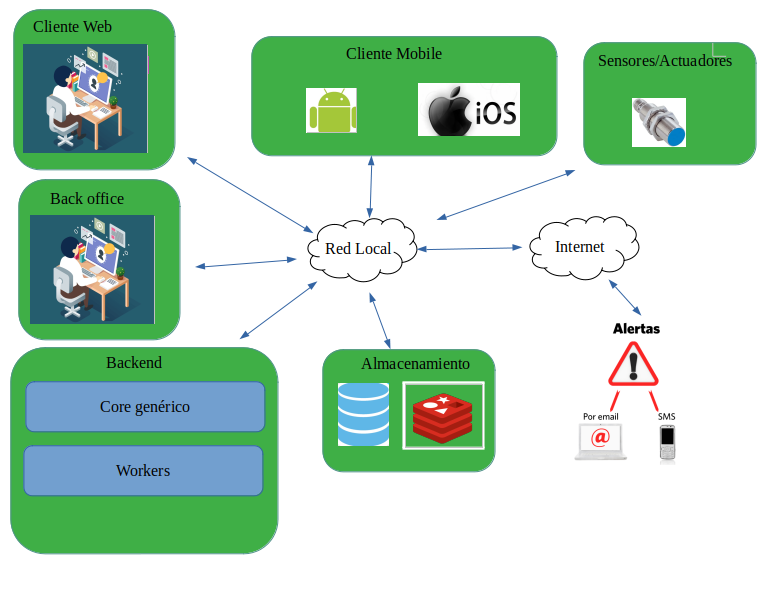
\includegraphics[width=.8\textwidth]{./Figuras/iot_nico.png}
\caption{Diagrama en bloques del sistema}
\label{fig:diagBloques}
\end{figure}

\section{2. Identificación y análisis de los interesados}
\label{sec:interesados}


\begin{table}[ht]
%\caption{Identificación de los interesados}
%\label{tab:interesados}
\begin{tabularx}{\linewidth}{@{}|l|X|X|l|@{}}
\hline
\rowcolor[HTML]{C0C0C0} 
Rol           & Nombre y Apellido & Organización 	& Puesto 	\\ \hline
%Auspiciante   &                   &              	&        	\\ \hline
Cliente       & Pablo Valentín Funes      & Funes - Ceriale Consultores en Ingeniería	& Ingeniero eléctrico\\ \hline
%Impulsor      &                   &              	&        	\\ \hline
Responsable   & \authorname       & FIUBA        	& Alumno 	\\ \hline
%Colaboradores &                   &              	&        	\\ \hline
Orientador    & \supname	      & \pertesupname 	& Director Trabajo final \\ \hline
%Equipo        & miembro1 \newline 
%				miembro2          &              	&        	\\ \hline
%Opositores    &                   &              	&        	\\ \hline
%Usuario final &                   &              	&        	\\ \hline
\end{tabularx}
\end{table}


\section{3. Propósito del proyecto}
\label{sec:proposito}

El propósito de este proyecto es generar una plataforma IOT multipropósito. La plataforma servirá de base para futuros trabajos de ingeniería, proporcionándole al alumno los conocimientos básicos para desarrollarse en los proyectos que puedan surgir.\\
Estos trabajos consistirían en la configuración de la plataforma para el cliente, con la posibilidad de integrar los distintos equipos en la plataforma como un servicio de ingeniería o un servicio de inteligencia y análisis de datos. 

\section{4. Alcance del proyecto}
\label{sec:alcance}

El proyecto incluye el desarrollo de un sistema encargado de:
\begin{enumerate}
\item Proveer una interfaz de usuario mobile (ios/android).
\item Proveer una interfaz de usuario web.
\item Proveer una interfaz de configuración web back office para administrar las funcionalidades según el cliente.
\item Registrar de forma persistente la información obtenida.
\item Generar alertas según parámetros establecidos.
\item Registrar las mediciones realizadas por sensores y actuadores.
\item Desarrollo del firmware en nodos sensores/actuadores para banco de pruebas.
\item Desarrollo del hardware en nodos sensores/actuadores para banco de pruebas.
\item Pruebas sobre la plataforma utilizando sensores de temperatura/humedad DHT22 como variables de entrada y 2 leds cumpliendo el rol de variables de salida.
\end{enumerate}

El proyecto no incluye:
\begin{enumerate}
\item Contratación de servicios de terceros.
\item Desarrollo de hardware de adquisición de datos.
\item Desarrollo de firmware para el hardware de adquisición de datos.
\item Desarrollos para las plataformas de Apple.
\end{enumerate}

\section{5. Supuestos del proyecto}

Para el desarrollo del presente proyecto se realizan los siguientes supuestos:
\begin{itemize}
	\item Se dispondrán los recursos económicos suficientes para adquirir los componentes necesarios para el banco de pruebas.
	\item Se dispondrá de los recursos necesarios para realizar la investigación de los recursos a emplear durante el proyecto.
	 \item Se dispondrá el apoyo de los orientadores a lo largo del proyecto.
	 \item Se dispondrá un alcance de las funcionalidades acorde al tiempo estipulado del proyecto (1 año).
\end{itemize}

\section{6. Requerimientos}
\label{sec:requerimientos}

A continuación se muestran los requerimientos del proyecto clasificados según el componente que tengan en común y la prioridad.
A menor valor numérico, la prioridad es mayor.

\begin{enumerate}
	\item Requerimientos interfaz cliente (web-mobile)
		\begin{enumerate}
			\item El sistema debe funcionar en los clientes web chrome y mozilla.
			\item El sistema debe funcionar en ios/android. 
			\item El usuario debe poder listar todos los sensores disponibles.
			\item El usuario debe poder visualizar las mediciones de los sensores disponibles.
			\item El usuario debe poder accionar un actuador en caso de contar con los permisos.
		\end{enumerate}
	\item Requerimientos del backoffice
		\begin{enumerate}
			\item El usuario debe poder ingresar mediante un login.
			\item El sistema debe permitir la configuración de las funcionalidades disponibles.
			\item El sistema debe permitir la actualización de los parámetros de un usuario.
			\item El sistema debe permitir la actualización de los parámetros de un sensor.
			\item El sistema debe permitir la configuración de una alerta a partir de los parámetros de un sensor.
			\item Requerimiento 2 (prioridad menor)
		\end{enumerate}
	\item Requerimientos del backend
		\begin{enumerate}
			\item El sistema debe persistir la información de los usuarios.
			\item El sistema debe persistir la información de los sensores.
			\item El sistema debe poder informar con una alerta si es necesario.
			\item El sistema debe poder comunicarse con los protocolos http-mqtt.
		\end{enumerate}
	\item Requerimiento de testing.
		\begin{enumerate}
			\item El sistema debe disponer una suite de pruebas unitarias para asegurar el funcionamiento.
			\item El sistema debe disponer un banco de pruebas con sensores y actuadores.
			\item El sistema debe disponer una serie de pruebas de integración utilizando el banco de pruebas.
		\end{enumerate}
\end{enumerate}

\section{7. Historias de usuarios (\textit{Product backlog})}
\label{sec:backlog}

En esta sección se incluyen las historias de usuarios y sus correspondientes ponderaciones.

\subsection{Usuarios}
Como usuario quiero registrarme en la plataforma e ingresar con mi correo electrónico para garantizar la seguridad de mi información.
\begin{itemize}
	\item Dificultad: 3 - El registro del usuario involucra muchas horas para asegurar la autenticación del mismo.
	\item Complejidad: 8 - La integración con algún servicio externo puede volverse difícil y deben considerarse muchos casos borde.
	\item Riesgo: 5 - Se debe asegurar el mecanismo para corroborar la identidad al momento del registro del correo electrónico, generalmente se usan sms o email.
\end{itemize}
Story Points: 16

\subsection{Sensores disponibles}
Como usuario quiero poder visualizar el listado completo de los sensores disponibles para poder seleccionar el sensor de interés.
\begin{itemize}
	\item Dificultad: 3 - Involucra hacer el pedido de información al backend y seleccionar la forma de mostrar la información.
	\item Complejidad: 5 - Hacer un servicio que devuelva información contemplando todos los casos posibles.
	\item Riesgo: 2 - Se puede dar el caso de no obtener información con el servicio teniendo que manejar un caso excepcional.
\end{itemize}

Story Points: 10
\subsection{Mediciones de un sensor}
Como usuario quiero poder visualizar las mediciones de un sensor seleccionado para observar el correcto funcionamiento del sistema.
\begin{itemize}
	\item Dificultad: 3 - Involucra el pedido de información al backend y seleccionar la forma de mostrar la información.
	\item Complejidad: 5 - Hacer un servicio que devuelva información contemplando todos los casos posibles.
	\item Riesgo: 3 - Se puede dar el caso de no obtener información con el servicio teniendo que manejar un caso excepcional.
\end{itemize}

Story Points: 11
\subsection{Alarmas}
Como usuario quiero recibir notificaciones por la aplicación o correo electrónico en el caso de una alarma para conocer el estado actual del sistema.
\begin{itemize}
	\item Dificultad: 5 - Se requiere correr un proceso de fondo revisando la situación particular de cada sensor para accionar una alarma.
	\item Complejidad: 13 - Cada sensor es diferente por lo que cada alarma es diferente y requiere darle un comportamiento particular.
	\item Riesgo: 5 - Puedo que no se dispare una alarma y ocurra un problema.
\end{itemize}

Story Points: 23
\subsection{Información de los sensores}
Como usuario quiero recibir la información de los sensores por correo electrónico en formato csv para poder realizar un posterior análisis de datos.
\begin{itemize}
	\item Dificultad: 5 - Requiere la búsqueda de la información particular y el formato.
	\item Complejidad: 5 - Requiere enviar un archivo por un servicio externo.
	\item Riesgo: 3 - El archivo puede contener errores de formato y no enviarse.
\end{itemize}

Story Points: 13
\section{8. Entregables principales del proyecto}
\label{sec:entregables}


Los principales entregables del proyecto son:

\begin{itemize}
	\item Manual de uso 
	\item Video tutorial de uso.
	\item Software ejecutable de la aplicación.
	\item Informe de avance del proyecto.
	\item Memoria del proyecto.
\end{itemize}


\section{9. Desglose del trabajo en tareas}
\label{sec:wbs}


En esta sección se muestra el listado de tareas que forman parte del proyecto.
\begin{enumerate}
\item Planificación del proyecto (70 hs)
	\begin{enumerate}
	\item Realizar el plan del proyecto (40 hs)
	\item Realizar el estudio de viabilidad económica-financiera del proyecto (20 hs)
	\item Aprobación de la planificación(10 hs)
	\end{enumerate}
\item Investigación y selección de tecnologías. (56 hs)
	\begin{enumerate}
	\item Investigación y selección de las tecnologías en el desarrollo del software (32 hs)
	\item Investigación de protocolos http-mqtt (8 hs)
	\item Investigacion sobre herramientas de deploy(16 hs)
	\end{enumerate}
\item Configuración de la infraestructura del proyecto. (58 hs)
	\begin{enumerate}
	\item Configuración de las bases de datos (8 hs)
	\item Configuración de las instancias de backend (12 hs)
	\item Configuración de las instancias de frontend web (16 hs)
	\item Configuración de un servicio externo para las pruebas unitarias CircleCi o Travis (6 hs).
	\item Configuración de herramientas para el deploy de la aplicación (16 hs).
	\end{enumerate}
\item Desarrollo del backend. (72 hs)
	\begin{enumerate}
	\item Desarrollo del endpoint del listado de sensores (8 hrs)
	\item Desarrollo del endpoint de las mediciones de un sensor  (8 hs)
	\item Desarrollo del endpoint para el registro de un usuario (12 hs)
	\item Desarrollo del endpoint para el login de un usuario  (8 hs)
	\item Desarrollo del backoffice (16 hs)
	\item Desarrollo del software para comunicacion con los sensores (20 hs)
	\end{enumerate}
\item Desarrollo del frontend web. (70 hs)
	\begin{enumerate}
	\item Diseño de las vistas de la aplicación (32 hs)
	\item Desarrollo de la vista del login de un usuario (12 hs)
	\item Desarrollo de la vista de un menú principal con las funcionalidades (8 hs)
	\item Desarrollo de la vista del listado de sensores (12 hs)
	\item Desarrollo de la vista de las mediciones de un sensor (12 hs)
	\end{enumerate}
\item Desarrollo del frontend mobile. (70 hs)
	\begin{enumerate}
	\item Diseño de las vistas de la aplicación (32 hs)
	\item Desarrollo de la vista del login de un usuario (12 hs)
	\item Desarrollo de la vista de un menú principal con las funcionalidades (8 hs)
	\item Desarrollo de la vista del listado de sensores (12 hs)
	\item Desarrollo de la vista de las mediciones de un sensor (12 hs)
	\end{enumerate}
\item Testing. (60 hs)
	\begin{enumerate}
	\item Diseño de casos de prueba (8 hs)
	\item Generación de datos de prueba (4 hs)
	\item Diseño del hardware de pruebas (8 hs)
	\item Ejecución del esquema de pruebas (34 hs)
	\item Generar reporte de las pruebas (6 hs)
	\end{enumerate}
\item Validación. (40 hs)
	\begin{enumerate}
	\item Diseño de ensayos de validación (12 hrs)
	\item Ensayos de validación (28 hs)
	\end{enumerate}
\item Presentación del trabajo. (142 hs)
	\begin{enumerate}
	\item Redacción del informe de avance (10 hs)
	\item Redacción del tutorial de uso (8 hs)
	\item Redacción de la memoria escrita (100 hs)
	\item Elaboración de presentación final (24 hs).
	\end{enumerate}	
\end{enumerate}

El tiempo total estimado del proyecto es de 638 hs.


\section{10. Diagrama de Activity On Node}
\label{sec:AoN}

En esta sección se muestra el diagrama de Activity On Node del proyecto.

\begin{figure}[htpb]
\centering 
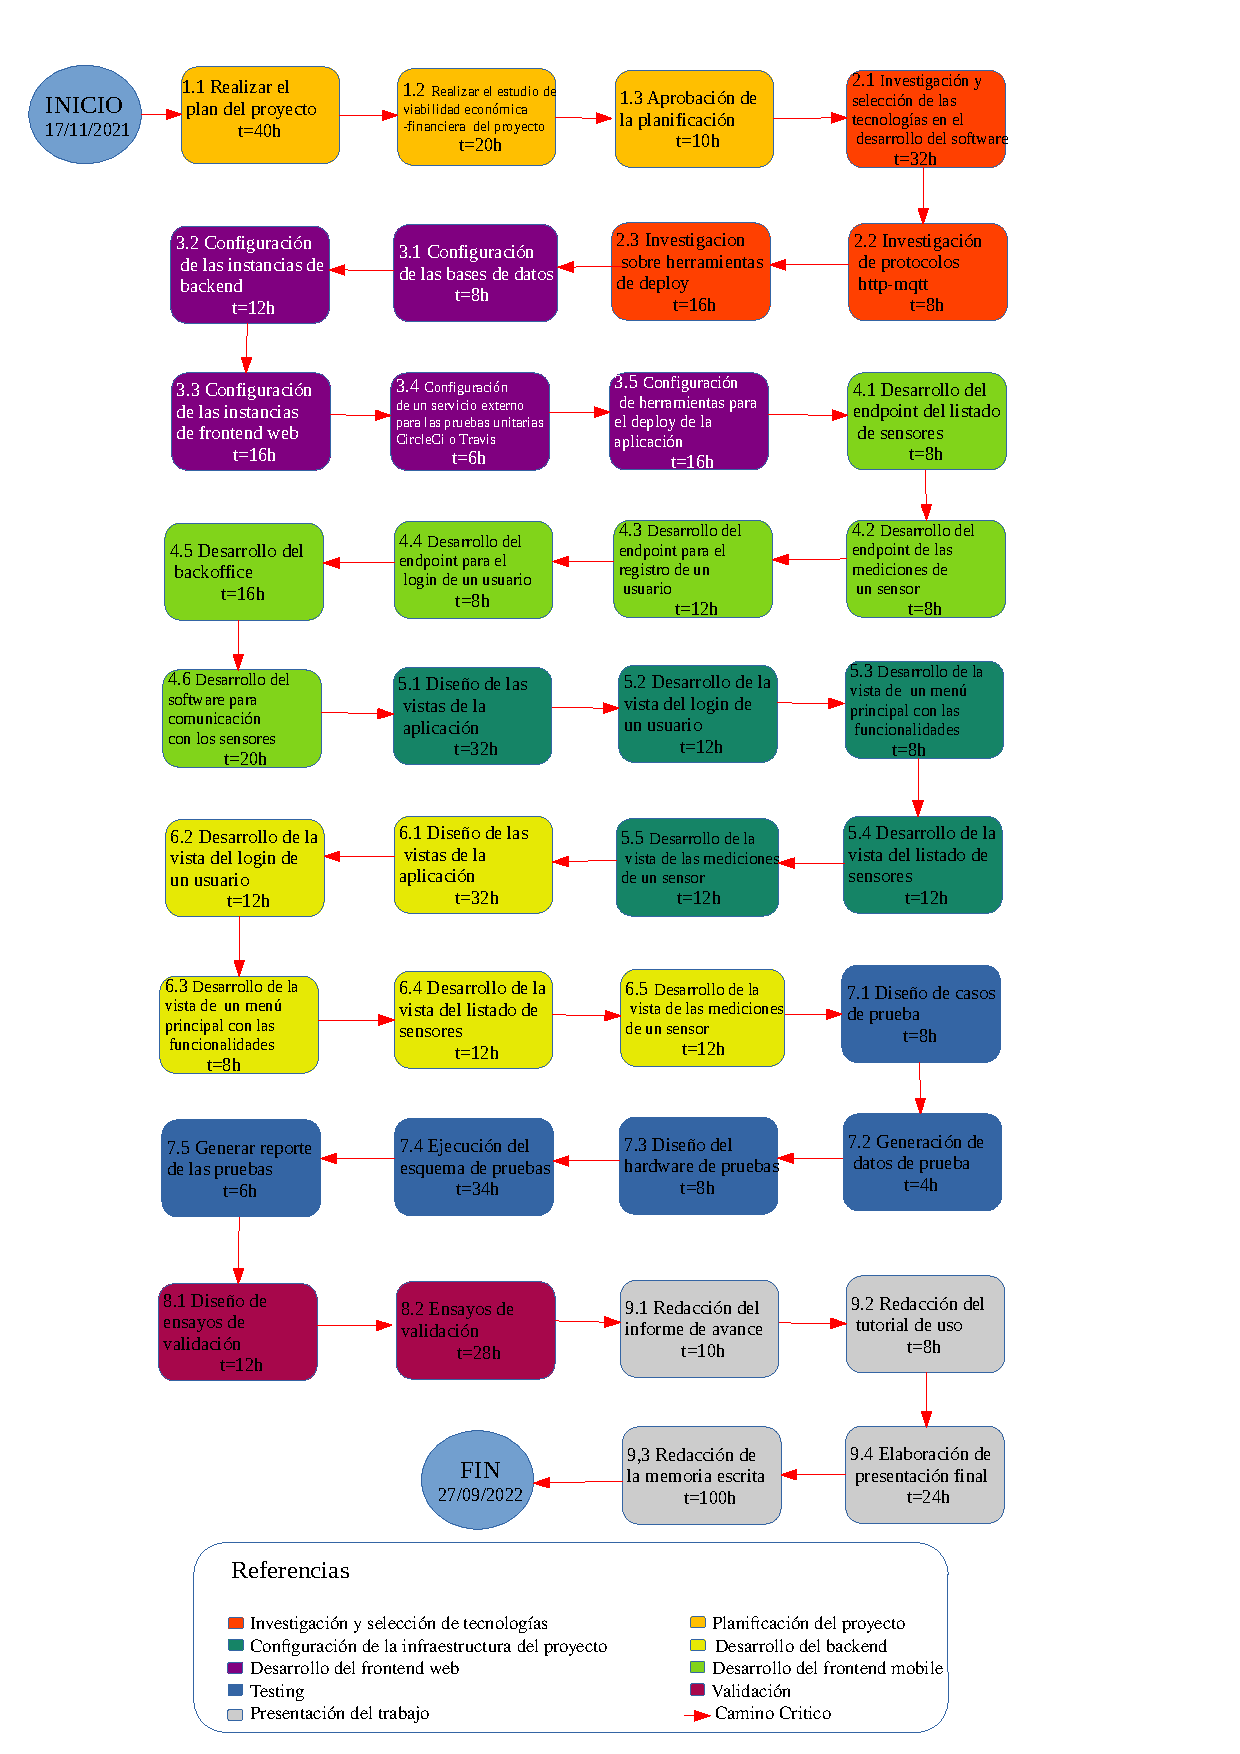
\includegraphics[width=1.0\textwidth]{./Figuras/aon_iot.pdf}
\caption{Diagrama \textit{Activity on Node} expresado en horas.}
\label{fig:AoN}
\end{figure}


\section{11. Diagrama de Gantt}
\label{sec:gantt}

En esta sección se muestra el diagrama de Gantt del proyecto.

\begin{landscape}
\begin{figure}[htpb]
\centering 
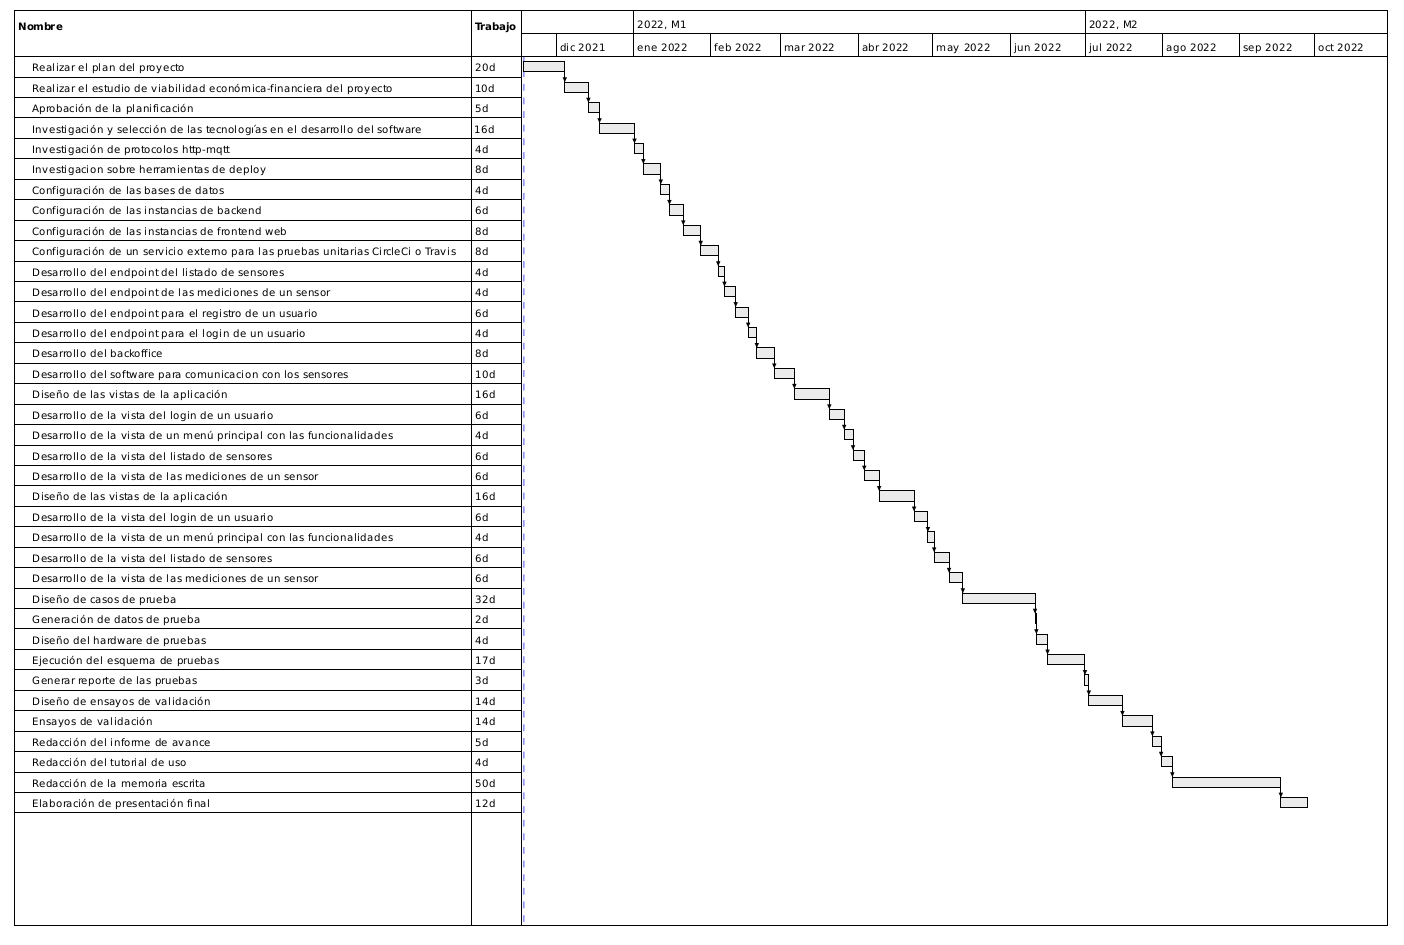
\includegraphics[angle=0,height=0.9\textheight]{./Figuras/gantt.png}
\caption{Diagrama de Gantt}
\label{fig:diagGantt}
\end{figure}
\end{landscape}


\section{12. Presupuesto detallado del proyecto}
\label{sec:presupuesto}
En esta sección se muestra el presupuesto del proyecto.

\begin{figure}[htpb]
\centering 
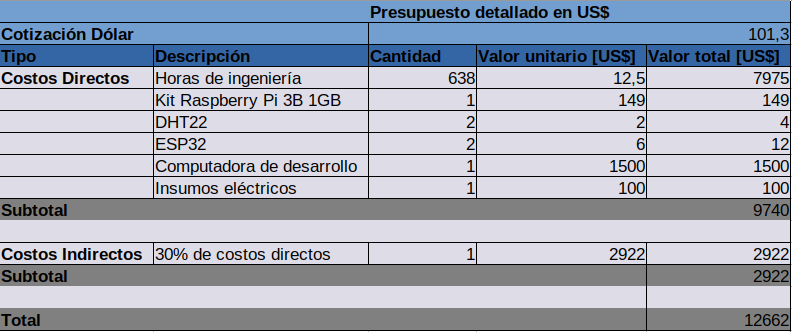
\includegraphics[width=1.0\textwidth]{./Figuras/presupuesto.png}
\caption{Presupuesto del proyecto en dólares.}
\label{fig:AoN}
\end{figure}

\begin{comment}

\section{13. Gestión de riesgos}
\label{sec:riesgos}

\begin{consigna}{red}
a) Identificación de los riesgos (al menos cinco) y estimación de sus consecuencias:
 
Riesgo 1: detallar el riesgo (riesgo es algo que si ocurre altera los planes previstos de forma negativa)
\begin{itemize}
	\item Severidad (S): mientras más severo, más alto es el número (usar números del 1 al 10).\\
	Justificar el motivo por el cual se asigna determinado número de severidad (S).
	\item Probabilidad de ocurrencia (O): mientras más probable, más alto es el número (usar del 1 al 10).\\
	Justificar el motivo por el cual se asigna determinado número de (O). 
\end{itemize}   

Riesgo 2:
\begin{itemize}
	\item Severidad (S): 
	\item Ocurrencia (O):
\end{itemize}

Riesgo 3:
\begin{itemize}
	\item Severidad (S): 
	\item Ocurrencia (O):
\end{itemize}


b) Tabla de gestión de riesgos:      (El RPN se calcula como RPN=SxO)

\begin{table}[htpb]
\centering
\begin{tabularx}{\linewidth}{@{}|X|c|c|c|c|c|c|@{}}
\hline
\rowcolor[HTML]{C0C0C0} 
Riesgo & S & O & RPN & S* & O* & RPN* \\ \hline
       &   &   &     &    &    &      \\ \hline
       &   &   &     &    &    &      \\ \hline
       &   &   &     &    &    &      \\ \hline
       &   &   &     &    &    &      \\ \hline
       &   &   &     &    &    &      \\ \hline
\end{tabularx}%
\end{table}

Criterio adoptado: 
Se tomarán medidas de mitigación en los riesgos cuyos números de RPN sean mayores a...

Nota: los valores marcados con (*) en la tabla corresponden luego de haber aplicado la mitigación.

c) Plan de mitigación de los riesgos que originalmente excedían el RPN máximo establecido:
 
Riesgo 1: plan de mitigación (si por el RPN fuera necesario elaborar un plan de mitigación).
  Nueva asignación de S y O, con su respectiva justificación:
  - Severidad (S): mientras más severo, más alto es el número (usar números del 1 al 10).
          Justificar el motivo por el cual se asigna determinado número de severidad (S).
  - Probabilidad de ocurrencia (O): mientras más probable, más alto es el número (usar del 1 al 10).
          Justificar el motivo por el cual se asigna determinado número de (O).

Riesgo 2: plan de mitigación (si por el RPN fuera necesario elaborar un plan de mitigación).
 
Riesgo 3: plan de mitigación (si por el RPN fuera necesario elaborar un plan de mitigación).

\end{consigna}


\section{14. Gestión de la calidad}
\label{sec:calidad}

\begin{consigna}{red}
Para cada uno de los requerimientos del proyecto indique:
\begin{itemize} 
\item Req \#1: copiar acá el requerimiento.

\begin{itemize}
	\item Verificación para confirmar si se cumplió con lo requerido antes de mostrar el sistema al cliente. Detallar 
	\item Validación con el cliente para confirmar que está de acuerdo en que se cumplió con lo requerido. Detallar  
\end{itemize}

\end{itemize}

Tener en cuenta que en este contexto se pueden mencionar simulaciones, cálculos, revisión de hojas de datos, consulta con expertos, mediciones, etc.  Las acciones de verificación suelen considerar al entregable como ``caja blanca'', es decir se conoce en profundidad su funcionamiento interno.  En cambio, las acciones de validación suelen considerar al entregable como ``caja negra'', es decir, que no se conocen los detalles de su funcionamiento interno.

\end{consigna}

\section{15. Procesos de cierre}    
\label{sec:cierre}

\begin{consigna}{red}
Establecer las pautas de trabajo para realizar una reunión final de evaluación del proyecto, tal que contemple las siguientes actividades:

\begin{itemize}
	\item Pautas de trabajo que se seguirán para analizar si se respetó el Plan de Proyecto original:
	 - Indicar quién se ocupará de hacer esto y cuál será el procedimiento a aplicar. 
	\item Identificación de las técnicas y procedimientos útiles e inútiles que se emplearon, y los problemas que surgieron y cómo se solucionaron:
	 - Indicar quién se ocupará de hacer esto y cuál será el procedimiento para dejar registro.
	\item Indicar quién organizará el acto de agradecimiento a todos los interesados, y en especial al equipo de trabajo y colaboradores:
	  - Indicar esto y quién financiará los gastos correspondientes.
\end{itemize}

\end{consigna}
\end{comment}


\end{document}
